\documentclass[12pt,a4paper,IEEEtran]{article}
\usepackage[utf8]{inputenc}
\usepackage{array}
\usepackage{amsmath}
\usepackage{amsfonts}
\usepackage{amssymb}
\usepackage{graphicx}
\usepackage{booktabs}
\usepackage{algorithm}
\usepackage{algpseudocode}
\usepackage{subcaption}
\usepackage[english]{babel}
\usepackage[export]{adjustbox}
\usepackage{enumerate}
\usepackage[left=3.5cm,right=2.5cm,top=2.5cm,bottom=2.5cm]{geometry}
\usepackage{lineno}
\usepackage{cite}
\usepackage{acronym}
\renewcommand{\baselinestretch}{1.5}



\begin{document}

	\begin{center}
		\begin{LARGE}			\bf{Identifying Deforestation using fair classical Image Processing Techniques\\}
		\end{LARGE}
		\vspace*{30pt}
		\textbf{Applied Digital Image Processing \\ Fall 2023}
		\vspace{40pt}
		
		\textbf{
			Shayan Shoaib Patel (Student ID: sp07101)\\
			Muhammad Areeb Kazmi (Student ID: mk07202 )\\
            Group 12}\\

		\vspace{30pt}
		
\includegraphics[width=0.3\textwidth]{./logo.png} \\
		\vspace{30pt}
		\textit{Under the kind guidance of}\\
		\textbf{Dr. Muhammad Mobeen Movania}\\
		\textit{\textbf{Assistant Professor, Computer Science}}
		
		
		\vspace{20pt}
		
		
		\textbf{Dhanani School of Science And Engineering\\
			Habib University\\
			December 10, 2023
		}
	\end{center}

\pagenumbering{arabic}

% Every latex document starts with a documentclass declaration like this
% The option dvips allows for graphics, 12pt is the font size, and article
%   is the style

%\usepackage[pdftex]{graphicx}
%\usepackage{url}

% These are additional packages for "pdflatex", graphics, and to include
% hyperlinks inside a document.

\setlength{\oddsidemargin}{0.25in}
\setlength{\textwidth}{6.5in}
\setlength{\topmargin}{0in}
\setlength{\textheight}{8.5in}

% These force using more of the margins that is the default style


% Everything after this becomes content
% Replace the text between curly brackets with your own


% You can leave out "date" and it will be added automatically for today
% You can change the "\today" date to any text you like


% \maketitle

% This command causes the title to be created in the document
\newpage
\section{Abstract}

\section{Introduction}
% this para is good. 
In the context of our present ecological challenges, addressing and raising awareness about global warming stands as a paramount imperative. Given the limitations in resources and the potential reluctance of governing bodies to prioritize this issue adequately, it becomes essential to pioneer a systematic approach for monitoring, reflecting upon, and mitigating these environmental changes. 

% can be used in significance of the research
Our primary objective is to institute a meticulous process for the collection and analysis of satellite imagery. Subsequently, we intend to apply various advanced methodologies and mathematical algorithms to these images. This multifaceted approach serves a dual purpose: it helps in our ability to fairly analyze and document alterations in land topography brought about by climate change upto an approximate degree, while also diminishing our reliance on local authorities and potential vested interests that may obstruct progress in this crucial area.
% significance

By implementing this approach, we aspire to foster greater transparency, accountability, and data-driven decision-making in the quest to combat global warming. Moreover, this initiative carries the potential to engage and enlighten the public about the pressing need for environmental conservation, ultimately leading to a more sustainable and resilient future for our planet as we try to compare and contrast different classical digital image processing techniques with the current state of the art method.
% An article style is separated into sections and subsections with 
%   markup such as this.  Use \section*{Principles} for unnumbered sections.


% \section{Motivation}
% The motivation behind the proposal is to work with a real world problem which is significant to the survival of human species.
% Deforestation is one of the by-products of the climate change that has contributed to the global warming. Keeping the context of
% the course in mind, we aim to use techniques and knowledge acquired in the course to try to improve the process of identifying deforestation and the effects brought
% by the anthropocene. 
% \newline The satellite technology accompanied with the high=resolution imagery can be a game changer in the monitoring and identification of deforestation and urban expansion.
Our project aims to utilize the capabilities and functionalities of classical digital image processing for the purpose mentioned above that can be done using satellite imagery and images from Google Earth.
% Here are some of the key motivations behind the project:
% \subsection[2.1]{Environmental Impact}
Deforestation is a major contributor towards
the global boiling, as environmentalists term it now (instead of global warming). The monitoring system can contribute towards helping the relevant stakeholders to make better informed decisions through sustainable development. \cite{thomas2023global}

% \subsection[2.2]{Utilizing the true essence of Computer Science}
% To our limited understanding, Computer Science has been the field of study that has been involved in solving problems that exist in the world. In fact, vast collaborations with practitioners, theorists, biologists, chemists, and people of other
% professions have led to the innovation of new tools, applications, and opportunities. The same analogy can be directed towards solving a part of the problem of climate change and deforestation. By deploying suitable machine learning algorithms, image classification, and object detection methods, if possible,
% we might be able to experience the very same essence of CS in this course.
% \newline  
% Apart from the technical aspects, the project will also give us the opportunity to pitch ideas to relevant stakeholders, conduct the various phases of the project by managing it on time, and improve our own skillset and knowledge arsenal.
% This project will help us to make a meaningful impact while gaining invaluable experience in the area of applied digital image processing.

\section{Literature Review}
This section entails a review of the previous work done in the scope of detecting deforestation using different types of satellite imagery. Most of the techniques use remote sensing, i.e., making use of the satellite imagery to detect image change and deforestation. While the methods in section 3.1 and 3.2 work on single band images, section 3.3 and onwards work on multi-band images which is the current state of the art procedure. \\
Our project aims to bring classical techniques and compare their results with the more accurate methods to see if the classical methods can be used to have a fair estimate of the deforestation since the acquisition of multi-band satellite imagery and the pre-processing required is cumbersome and cannot raise public awareness.

%Taken from Paper 3

%Taken from Paper 3

\subsection[3.1]{Image Clustering} 
Content Based Image Clustering (CBIR) is a method used to group or classify objects into different classes which have similar properties. These classifying of images help us study different characteristics of 

FCM (Fuzzy C-mean) \cite{BEZDEK1984191} is one of the most common form of image clustering and it is the based on the principle of fuzzy classification. In fuzzy C-mean clustering pixels with identical properties will be grouped into to same categories or clusters.

The input images of the fuzzy C-mean clustering, where Gray scale images and the cluster centers were computed automatically by the function itself. Once the cluster center was found and fixed, the next stage was setting the rules for fuzziification. That is if-then rules are given below assuming that the three cluster values are cluster 1, 2 and 3.
\begin{itemize}
	
	\item If pixel (i,j) is less than Cluster-1, center make it black(0)
		%\centering
	\item If pixel (i,j) is greater than cluster-3 center make it White (1).
		%\centering
	\item Else make pixel (i,j) in between black and white (0.5). 	
	%\end{flushleft}
\end{itemize}

The FCM algorithm continuously upgrades and moves this cluster centers iteratively to the ideal or right position. So by continuous moving of initial cluster centers, it precisely clusters the image into different regions and groups the accuracy of the membership grades of each groups [Cite3 in 23 in Doc]. 


\subsection[3.2]{Otsu Method on color spaces}
The Otsu Method \cite{5254345} is seperating or dividing of images into different clusters or regions based on common properties and/or differences between other regons properties. One property out of the many could be applied to separating images into regions is pixel intensity. 

So we normally can segment images into different regions through thresholding or separating the pixel levels into different scales. These different thresholding scales create different regions corresponding to the pixel intensity values. 
\newline A simple example can be thresholding a gray scale image pixels into two regions, by transforming the gray scale image into binary image, which will consist of only two regions, namely either the black or white.

If $G(x,y)$ is a threshold version of $f(x,y)$ at some global threshold $T$,:
\[G(x,y) =
\begin{cases}
1 & \text{if } f(x,y) \geq T\\
0 & \text{ otherwise}
\end{cases}
\]

This method has been used with color spaces like HSV (Hue, Saturation, Intensity), and L*a*b* to identify areas of deforestation that we will further see in the methodology section.


% paper 2 used

% \subsection[3.3]{Image ratioing}
% Ratioing is considered to be relatively rapid means of identifying areas of change. In ratioing two registered images from different dates with one or more bands in an image are ratioed, band by band. The data are compared on a pixel or pixel basis. 

% \begin{equation}
% R(x) = \frac{I_{1}(x)}{I_{2}(x)}
% \end{equation}

% If the intensity of reflected energy is nearly the same in each image of R(x)=1, this indicates no change. In areas of change, the ratio value would be significantly greater than one or less than one, depending upon the nature of the change between the two dates. 

% Paper 2 used

% \subsection[3.3]{Change Vector Analysis}
% The change vector analysis \cite{MINU20151366} involves two variables, the magnitude of variation and the angle of the change vector.
% The change vector is obtained by subtracting the images represented in vector form.
% The first step of the CVA method is to find (Normalized Difference Vegetation Index) NDVI and (Bare Soil Index) BI values of both the images.

% \begin{equation} NDVI = (NIR - RED) / (NIR + RED) \end{equation}
% \begin{equation}
% 	BI = ((SWIR + RED) - (NIR + BLUE)) / ((SWIR + RED) + (NIR + BLUE))
% \end{equation} 
% where $NIR$, $RED$, $SWIR$ and $BLUE$ are the spectral reflectance measurements acquired in the near-infrared, red, short wave infrared and blue regions.
% Change vector of each pixel includes two components NDVI and BI, which are the 2 axes in Cartesian coordinate system. The start point and finish point of the change vector are the locations of pixel in NDVI-BI space. The magnitude of vector represents the change intensity and the direction of vector represents the change dimension 
% Further calculations not only allow us to furhter divide the values into two different groups which do not only allow to see the land and forestation/plantation affected.

% \subsubsection[3.4.1]{Tasseled Cap Transformation Method}
% The tasseled cap transformation parameters of ETM+ imagery were used to calculate the Brightness, Greenness 
% and Wetness components of each image. The Tasseled cap transformation coefficients derived for Landsat 7 ETM+ 
% data by the EROS Data Center (Huang et al. 2002) are given in Table 2. Brightness is a weighted sum of all bands, 
% defined in the direction of the principal variation in soil reflectance. Greenness is a contrast between the near infrared and visible bands. It is strongly related to the amount of green vegetation in the scene. Wetness relates to 
% canopy and soil moisture. The brightness, greenness and wetness indexes are obtained for both the images.

% \begin{figure}[h]
% 	\centering
% 	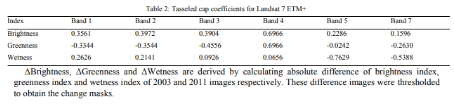
\includegraphics[width=0.7\linewidth]{./tasseledcap}
% 	% \caption{Tasseled Cap Transformation}
% 	\label{fig:tasseledcap}
% \end{figure}

% \subsubsection[3.4.2]{Principal Component Analysis Method}
% The principal components transformation is a linear transformation which defines a new, orthogonal co-ordinate 
% system such that the data can be represented without correlation. A bi-temporal feature space is constructed by 
% placing the two image vectors in the same space. The transformation is found from the eigen vectors of the 
% covariance matrix of the original data. Each individual pixel is transformed by vector multiplication of its original 
% vector and the eigen vectors, resulting in coordinates in the new space. The transformed data is re-arranged back into
% wo images corresponding to the first and second principal components. The first component images contain no change pixels whereas the second component images contain change information between the different dates.

% Therefore, using the Brightness, Greenness and Wetness components of each image, the change vector analysis was performed. 

%Paper 9 used here

\subsection[3.3]{NDVI Method}
The Normalized Difference Vegetation Index (NDVI) is widely employed for vegetation assessment by gauging the abundance of vegetation cover on land. The principle underlying NDVI hinges on the capacity of chlorophyll in plants to absorb red and blue light while reflecting near-infrared (NIR) and green light. Landsat imagery, sourced from diverse satellites, particularly Landsat 7 and 8, has been instrumental in acquiring data for the wavelengths absorbed by vegetation. With an operational history spanning over two decades, Landsat satellites have been optimized to furnish data primarily centered on land cover and vegetation dynamics based on surface reflectance. 

The utilization of Surface Reflectance products further refines this process by providing an estimate of spectral reflectance at ground level, effectively negating the impact of atmospheric scattering or absorption that could otherwise distort measurements. This approach ensures the accuracy and reliability of NDVI data in discerning variations in vegetation over time. The Landsat were further the preferred choice as among the many other satellites with the same idea developed for monitoring the land changes, Landsat is the only of the few remaining satellites which has the data for such an extended time. 

Originating in the 1970s, the utilization of the Normalized Difference Vegetation Index (NDVI) has undergone a transformative evolution. Initially designed for vegetation detection, it has progressed to become an invaluable tool for monitoring and predicting vegetation health and growth. This comprehensive methodology has found substantial application in environmental monitoring, notably in the Brazilian forest [3]. Employing the Random Forest model, historical NDVI data has been meticulously analyzed to not only comprehend the past growth patterns of the Brazilian forest but also to project future developments. Using the GEEE platforms to extract the utilize the data available, the data was then processed and checked against the Random Forest algorithm to monitor the changes over the years, and see the future vegetation prospects based on this idea.  

The versatility of NDVI extends to pattern monitoring, exemplified by the Mimbo forests [4]. In this context, the NDVI method served as a robust metric for quantifying deforestation. Incorporating regression analysis into the evaluation of identified patterns has not only facilitated a nuanced understanding of past deforestation trends but also augments the capability to predict future vegetation dynamics within the Mimbo region. 

 

% This method entails the use of multi-band satellite imagery to detect and produce results for areas of vegetation \cite{isprs-annals-IV-4-W4-379-2017} where the Landsat 8 has eight bands: blue, green, red, near-infrared 1, 
% near-infrared 2, thermal, mid-infrared, panchromatic. All of the 
% bands have 30 meters resolution, except thermal with 60 and 
% panchromatic with 15 meters of resolution (GIS Geography, 
% 2017, USGS, 2017)
% \newline Picked bands of the imagery are band 2, 
% band 3 and band 4, representing, green, red and near infrared 
% bands. These bands are selected since they are used in the 
% calculation of the NDVI. NDVI calculation is shown in equation below:
% \begin{equation}
% NDVI = \frac{NIR - RED}{NIR + RED}
% \end{equation}
% where $NIR$ and $RED$ are the near infrared and red bands respectively.
% \newline Cropped images of these three bands are combined to form a 
% false color composite image. 
% Three other metrics are used, namely accuracy, precision, and recall.

% Recall metric represents the rate of 
% the correctly identified vegetated regions and calculated as TP / 
% (TP + FN). On the other hand, precision indicates what 
% percentage of the regions found as vegetation are actually true 
% with respect to ground truth and calculated as TP / (TP + FP). 
% Using precision and recall, we can calculate an fScore value for 
% prediction of vegetated regions, which is a score varies in [0, 1] 
% range. The higher the score value, the better the result is. The 
% formula for fScore is shown in equation 3.

% \begin{equation}
% fScore = \frac{2 * Precision * Recall}{Precision + Recall}
% \end{equation}

% where Precision is the precision value for the case, Recall is the recall value for the case, and $fScore$ is the resultant $fScore$ that shows how good the result is.

% Moreover, the vegetation ratio is also used to examine the loss in vegetation areas. Here, the total number of pixels with value 1 are divided by the total number of pixels.
% \begin{equation}
% Vegetation Ratio = \frac{Total Number of Pixels with Value 1}{Total Number of Pixels}
% \end{equation}

%Paper 1 used here

% \subsection[3.5]{Wavelength Method}
% The data was processed and the analysis was by determining the wavelengths of certain frames from Landsat-7 and four frames from Landsat-8. The bands were combined for each frame and the null values were eliminated using the Copy Raster toolset. Finally, mosaicing was done on the frames for each year separately using the Mosaic to New Raster tool.
% \newline The spatial-temporal variability
% of normalized difference vegetation index NDVI was assessed to study deforestation using harmonic
% analysis. We first spatially normalized observations to reduce seasonality. Subsequently, we detected
% deforestation by assessing whether a newly acquired observation (satellite image) in the monitoring
% period is in an extreme change when compared against spatially normalized values in present time data
% defined over a reference period. The calculation of the NDVI for multi-date satellite images of Landsat
% (7, 8) was used to perform change detection of the deforestation in Huambo Miombo.
% \newline The
% NDVI, as one of the most successfully used vegetation spectral indices, allows comparison between
% inter-annual and seasonal changes in vegetation. The NDVI measures the amount of green vegetation
% in an area and is used to distinguish forested from deforested areas.

% \begin{figure}[h]
% 	\centering
% 	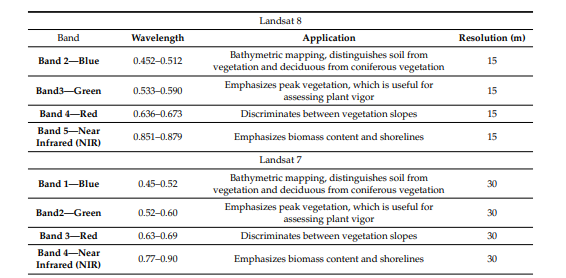
\includegraphics[width=0.7\linewidth]{./wavelength-9.png}
% 	\caption{Landsat Satellite Sensor characteristics}
% 	\label{fig:wavelength}
% \end{figure}

\section{Methodology}
As undergraduate students with limited knowledge and expertise, we were not able to come up with a novel idea. However, keeping in mind the techniques learned in the course of Applied Digital Image Processing, we implemented the methods that have been used for detecting deforestation in the papers cited above.

\subsection[4.1]{Image Clustering}
This classifying of images into groups help assist study different characteristics of the image like better flow, pattern changes and similarity of events or phenomenon. Further clustering of images gives clusters or regions with detailed and concise information and the content of the images which ease the task of asserting this regions of clusters. 
\newpage The Fuzzy C-Means (FCM) clustering method \cite{BEZDEK1984191} is based on minimizing the following objective function:
\begin{equation}
J_m = \sum_{i=1}^{n} \sum_{j=1}^{c} u_{ij}^m \cdot \|\mathbf{x}_i - \mathbf{v}_j\|^2
\end{equation}
\newline Here's a breakdown of the terms:
\begin{itemize}
    \item $J_m$ is the objective function to be minimized.
    \item $n$ is the number of data points.
    \item $c$ is the number of clusters.
    \item $u_{ij}$ is the degree of membership of data point $\mathbf{x}_i$ to cluster $j$.
    \item $m$ is a weighting exponent, usually set to 2 for FCM.
    \item $\mathbf{v}_j$ is the centroid of cluster $j$.
    \item $\|\mathbf{x}_i - \mathbf{v}_j\|^2$ is the Euclidean distance between data point $\mathbf{x}_i$ and the centroid $\mathbf{v}_j$.
\end{itemize}

The objective is to find the membership values \( u_{ij} \) and cluster centroids \( \mathbf{v}_j \) that minimize the objective function. The degree of membership \( u_{ij} \) indicates the fuzzy assignment of data point \( \mathbf{x}_i \) to cluster \( j \), with higher values indicating stronger membership.


% We acquired the satellite images from Google Earth Pro that is available for free from Google. For the multiple band images, we used Landsat 8 images from the USGS Earth Explorer website. The images were downloaded in the GeoTIFF format and were used for further processing. The images taken and uploaded on our Github repository are from the rural and urban areas of Sindh. 

\subsection[4.2]{Otsu Method}
The method involves finding an optimal threshold that minimizes the intra-class variace of pixel intensities:
\begin{equation}
	\sigma^2_w(t) = w_1(t) \cdot \sigma_1^2(t) + w_2(t) \cdot \sigma_2^2(t)
\end{equation}
Where: 
\begin{enumerate}
	\item $t$ is the threshold value.
	\item $\sigma^2_w(t)$ is the weighted sum of the variances of the two classes spearated by the threshold
	\item $w_1(t)$ and $w_2(t)$ are the probabilities of the occurences of the two classes separated by the threshold.
	\item $\sigma_1^2(t)$ and $\sigma_2^2(t)$ are the variances of the two classes separated by the threshold.
\end{enumerate}
The goal here, is to find the threshold value $t$ which effectively spearates the image into two classes, that minimizes the intra-class variance and maximizes the inter-class variance. \cite{5254345}

% When it comes to images obtained from Google Earth Pro, we applied Fuzzy C-Mean Clustering (refer to Section 3.1) and Otsu thresholding (refer to section 3.2) separately. 

% For the multi-band images, we used the NDVI method (refer to section 3.4) and the Wavelength method (refer to section 3.5) separately.

\subsection[4.3]{NDVI Method}
The implementation of the NDVI ratio to check the absorbed and reflected wavelengths from a particular region and is then used for the formula  
\begin{equation}
	NDVI = (NIR - RED) / (NIR + RED)
\end{equation}

Where $NIR$ corresponds to the near-infrared wave. These individual wavelengths are calculated at each point for a pixel and is then used to monitor the type of vegetation. The $NDVI$ yields a value ranging from -1 to 1 where -1 – 0 indicated dead plants or inanimate objects, 0 – 0.33 are considered as healthy plants, 0.33 – 0.66 were considered as moderately healthy plant and 0.66 – 1 were considered as healthy plants.  
 
Utilizing these values the previous approaches as mentioned plotted an image identifying the regions which had a healthy vegetation and which did not. Different images for each time were generated and showed as a visual representation to the console. 

 

% For comparing the results produced by the methods above, we used accuracy parameters and visual observation to determine the best method. The accuracy parameters used were precision, recall, and fScore. The visual observation was done by comparing the results produced by the methods with the ground truth images.

% We also used parameters like timing the execution or running time of our programs to see which program runs faster. 
\section{Implementation}
The implementation of the sections discussed below can be found on our Github repository \cite{adip_group_project}
\subsection{Image Clustering}
Our code implements the Fuzzy C-Means (FCM) clustering algorithm for image segmentation, focusing on feature detection, especially in identifying vegetation. We start by initializing a membership matrix, a crucial part of FCM, where each entry signifies the pixel's association degree with each cluster, capturing the uncertainty in pixel assignments during clustering. The iterative refinement of cluster centers and the membership matrix is then executed through a structured process.  

%Initially, cluster centers are set by randomly selecting data points from input samples (X), and the membership matrix is initialized using the initialize membership_matrix_function. This function assigns and normalizes random values, ensuring they collectively sum to 1 for each data point. The iterative phase continues until convergence or a specified number of iterations. In each iteration, the cluster centers are updated through the update_cluster_centers function, calculating new centers based on the current membership matrix, input data (X), and a fuzziness parameter. Simultaneously, the update_membership_matrix function recalculates the membership matrix based on the updated cluster centers, input data (X), and the fuzziness parameter. Convergence is determined by assessing changes in cluster centers and the membership matrix against a defined tolerance. If criteria are met, the algorithm terminates; otherwise, it continues. The final output consists of refined cluster centers and a membership matrix, capturing patterns within the input data. This ensures the algorithm stops iterating when updates reach a satisfactory precision level.
Initially, cluster centers are set by randomly selecting data points from input samples (\(X\)), and the membership matrix is initialized using the initialize \\membership\_matrix\_function. This function assigns and normalizes random values, ensuring they collectively sum to 1 for each data point. 
The iterative phase continues until convergence or a specified number of iterations. In each iteration, the cluster centers are updated through the \texttt{update\_cluster\_centers} function, calculating new centers based on the current membership matrix, input data (\(X\)), and a fuzziness parameter.

Simultaneously, the \texttt{update\_membership\_matrix} function recalculates the membership matrix based on the updated cluster centers, input data (\(X\)), and the fuzziness parameter. Convergence is determined by assessing changes in cluster centers and the membership matrix against a defined tolerance. If criteria are met, the algorithm terminates; otherwise, it continues. The final output consists of refined cluster centers and a membership matrix, capturing patterns within the input data. This ensures the algorithm stops iterating when updates reach a satisfactory precision level.

The update of cluster centers involves computing a weighted average of data points based on the membership matrix, while the membership matrix is updated by recalculating the degree of association between data points and clusters. Convergence is determined by evaluating changes in cluster centers and the membership matrix. In image processing, the code utilizes the LAB color space, extracting the L channel representing luminance. The L channel's pixel values are rescaled and used as input for FCM clustering, resulting in a segmented image. The code further aids in identifying areas with high intensity, indicating potential vegetation. Overall, this implementation clarifies the FCM algorithm's application in image segmentation. 

\subsection{Otsu Method}
The provided code utilizes the Otsu thresholding method to segment images in different color spaces: HLS (Hue, Saturation, Intensity), HSV (Hue, Saturation, Value), and LAB (Luminance, Green-Red, Blue-Yellow). The algorithmic explanation for the Otsu method in each color space is detailed below: 

HLS Color Space: The code begins by converting the input image to the HLS color space and then splits it into three channels: Hue (H), Saturation (S), and Intensity (I). Otsu thresholding is independently applied to each channel, determining optimal threshold values based on the channel's pixel intensity histogram. Binary images are created for the Hue and Saturation channels, showcasing the segmented regions. 

HSV Color Space: Similarly, the input image is converted to the HSV color space, and the image is split into three channels: Hue (H), Saturation (S), and Value (V). Otsu thresholding is individually applied to each channel, leading to the creation of binary images. The resulting segmented regions are displayed for the Hue and Saturation channels. 

LAB Color Space: The code then proceeds to convert the input image to the LAB color space, splitting it into three channels: Luminance (L), Green-Red (a), and Blue-Yellow (b). Otsu thresholding is independently applied to each channel, determining optimal thresholds based on pixel intensity histograms. Binary images are generated for the Luminance, Green-Red, and Blue-Yellow channels, displaying the segmented regions. 

In each color space, the Otsu thresholding method is employed to find optimal thresholds that maximize variance between foreground and background pixel classes. The resulting binary images highlight segmented regions, providing a visual representation of the segmentation outcomes. 

Additionally, the code includes post-processing steps where the segmented regions meeting specific criteria are highlighted in red. This enhancement offers a clearer visual indication of the identified segmented areas. 

\subsection{NDVI Method}
Two TIF files, corresponding to different spectral bands of satellite imagery, are loaded using the \texttt{rasterio} library. The red and near-infrared (NIR) bands are read as NumPy arrays, denoted as \texttt{red\_band} and \texttt{nir\_band}.

The script computes the band difference by subtracting the NIR band from the red band, resulting in the band difference. Additionally, the script determines the dimensions (height and width) of the image.

Using \texttt{np.any()}, the code checks for non-zero values in the red band. If non-zero values are present, the script identifies the index of the first non-zero value.

NDVI is calculated using the equation 3 in Section 4.3.
The NDVI values are clipped to ensure they fall within the range \([-1, 1]\). A threshold value (e.g., 0.2) is defined to distinguish areas with high and low NDVI values.

Binary masks, namely \texttt{high\_ndvi\_mask} and \texttt{low\_ndvi\_mask}, are created to highlight areas with high and low NDVI values based on the defined threshold.

Images are generated to highlight areas with high and low NDVI separately. High NDVI areas are depicted in green, and low NDVI areas are depicted in red in the respective highlight images.

The script combines the high and low NDVI highlight images into a single RGB image (\texttt{highlight\_image}). In this representation, high NDVI areas appear in green, low NDVI areas in red, and other areas in black.

This script effectively processes satellite imagery, calculates NDVI, and visually represents areas with varying levels of vegetation health.


\section{Experimental Results}
Each of our code were executed and timed appropiately. Where analysis was done not by only varying the parameter values but also working principle of each code with varying image types and the type of landscape provided to it as well. Each method would be discussed and the type of result that it had provided with. 

The Clustering method had a controllable factor of the number of clusters which would be required to be taken for.  Increasing the number of clusters would only increase the amount of variations of the classes of pixels to be grouped and formed for the image. This would lead to an inconsistency as the code works on the idea of the green pixels being seperately and would lead to the different shades of green being grouped in different clusters. Where if we were to take this for different images, each would lead to a different normalized binary value. Thus, standardization would not only be hard but also difficult to maintain without using a machine learning model where for a large data set it would be trained for and then checked against each. Figure 1a below shows when we use the number of clusters to be 6 and followed by 1b showing the same image but for 3 number of clusters. Thus, after more trial and errors, 3 was found to be the closest number of clusters for which the most accurate clustering method could be deployed with the best vegetation detection possible.  

\begin{figure}[ht]
    \centering
    \begin{subfigure}{0.45\textwidth}
        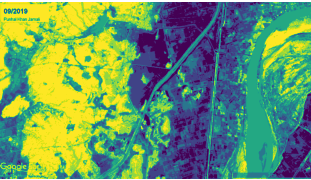
\includegraphics[width=\linewidth]{fig1a.PNG} % Replace 'image1' with your actual filename
        \caption{Caption for Figure 1a}
        \label{fig:subfig1}
    \end{subfigure}
    \hfill
    \begin{subfigure}{0.45\textwidth}
        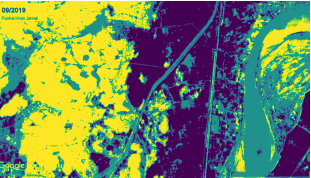
\includegraphics[width=\linewidth]{fig1b.PNG} % Replace 'image2' with your actual filename
        \caption{Caption for Figure 1b}
        \label{fig:subfig2}
    \end{subfigure}
    \caption{Overall caption for both figures.}
    \label{fig:overall}
\end{figure}

However an important point to further note is also the idea of image and its resolution. A low resolution image could result in the mixture of clusters where different pixels could be grouped for the wrong clusters leading to a little deviation of identifying the wrong area for the vegetation. Such as in fig 2 below where different areas were being identified as the area of vegetation even though they were not (extra areas marked with red). 



The NDVI method was the most reliable method as discussed before due to its implementation being reliant on extremely accurate information provided by the satellite. However, for an individual to only include a diagram or to get a rough estimate would be required to extract the information by first getting the individual bands. The file size of the images themselves are very large due to the aspect of high quality data as compared to the clustering method where only a screen shot would also suffice, the process of getting the data would be a little hard to navigate. Followed by the selection of the satellite and ensuring the given satellite would have the up to date data or not. Where the time taken to handle each data image would almost near to the time being taken by clustering. 

Thus this results in the following analysis for each of the methods below where the time taken for each to run is shown below  

\begin{table}[h]
	\centering
	\begin{tabular}{|l|c|}
	\hline
	\textbf{Method Used} & \textbf{Time Taken for CPU (s)} \\
	\hline
	NDVI & 12.5625 \\ 
	\hline
	Clustering & 12.421875 \\ 
	\hline
	Otsu & 0.015625 \\
	\hline
	\end{tabular}
	\caption{Time taken for different methods on CPU.}
	\label{tab:methods_time}
\end{table}
	
It is observable based on the table 1 above where the time taken for each NDVI and Clustering is almost equal, clustering would still be giving an estimate as compared to the NDVI method. However based on the technique and idea used to get information and the idea of automation, clustering would give a good estimate while having the idea of getting incorporated with automation tasks which involve only taking the screen shot of the map as compared to NDVI where automation would also be complicated as the selected files would have to contain the required bands. Thus, both the ideas could also be used to track forestation as seen in fig 4 where the red area identifies the area of deforestation and blue identifies the area of afforestation. Where with some additional changes, it could further be improved to the extent where the area of deforestation and afforestation could also be found. 

The Otsu method would not be regarded in this case as the idea of Otsu revolves around the varying image properties where it was for varying images different channels were being to identify the area of forestation or not and relied heavily on the user identifying which would be more appropiate rather than the idea of automating it for any image it would be given. Thus, even though it would be useful in some aspects but in the larger aspect it would not be useful to us.  
 
% add system specifications on which the results are run


\section{Conclusion}

\section{Acknowledgements}
We thank our course instructor, Dr. Muhammad Mobeen Movania, for his guidance and support throughout the course. 

\bibliographystyle{IEEEtran}
\bibliography{references.bib}

Citations for NDVI and intext too. Also, cite the 3rd paper and others
\end{document}